\documentclass{article}

\usepackage{amsmath}
\usepackage{graphicx}

\addtolength{\oddsidemargin}{-.3in}
\addtolength{\evensidemargin}{-.3in}
\addtolength{\textwidth}{0.6in}

\begin{document}

\title{Homework 4\\
       Parallel Sort}
\author{Geoffrey Ulman\\
        CSI702}
\date{March 2010}
\maketitle

\section{Design}
My serial sort is a simple quick sort implementation. My parallel sort is a bin sort very similar to the implementation analyzed in our previous homework. Each node receives an equal portion of the data set from node 0. Node 0 then calculates bin boundaries by selecting a small subsample of the entire data set, sorting it, and choosing data elements from it at regular intervals. This is done as an attempt to reduce communications by making the amount of data which ends in each bin as even as possible. Node 0 then informs the other nodes of the bin values it has chosen. The nodes then bin their local data and send the bins to the appropriate nodes. The nodes then perform local serial sorts on their subset of the data and send the results back to node 0.

\section{Challenges}
Writing a correct and efficient serial sort was a non-trivial challenge because I did not want to simply use the sort function built into the c standard library. I chose binary sort as my serial sort. My implementation works in place, but is not necessarily a stable sort. It also does not switch to a simpler sort for efficiency when the size of the recursive sub-problems becomes small.

Debugging my parallel implementation was also quite difficult. My communication logic was relatively straightforward and no serious debugging was needed there. What proved difficult was tracking down memory allocation problems which arose because of the somewhat complicated bookkeeping necessary to keep track of how much data had been stored in each bin. Originally, each processor allocated enough space in each bin for the entire data set (for simplicity). However, for large data sets and large numbers of nodes I began running into memory errors. This took a significant amount of trial and error to find.

After fixing the bugs described above, my parallel implementation worked, but was quite slow. For simplicity, I was using far too much synchronous communication. My first implementation had the nodes sending their binned data to each other essentially one node at a time. The current implementation has all the nodes send their binned data to all other nodes asynchronously.

This problem was the first time that I had worked with variable sized messages in MPI, so I had to familiarize myself for some of the functions for retrieving data from \verb!MPI_Request! and \verb!MPI_Status! objects as well as think through the logic necessary to combine the data from multiple variable sized messages into a single array. 

Finally, I was not able to profile the code for arrays larger than \(10^9\) because the messages I was attempting to send exceeded the maximum message size. To experiment further with such large data sets would have required even more complicated algorithms to split up messages as they got too large. 

\section{MPI Commands}
Like all MPI programs, the commands \verb!MPI_Init!, \verb!MPI_Comm_size!, \verb!MPI_Comm_rank!, and \verb!MPI_Finalize! were used to initialize and get basic information about the MPI environment. Unsorted segments of data was distributed to nodes using \verb!MPI_Isend! and \verb!MPI_Waitall! was used by node 0 to wait for the sends to complete. Because binning was calculated on the host node, \verb!MPI_Bcast! was used to distribute the bin edges to the other nodes. Data was sent using \verb!MPI_Isend! and both \verb!MPI_Irecv! and \verb!MPI_Recv! were used for receiving data. Synchronous receives were used when receiving unknown quantities of data from multiple nodes. This greatly simplified the task of collecting the data into a single array for processing. \verb!MPI_Probe! and \verb!MPI_Get_count! were also very important for handling messages of unknown size.

\section{Performance Analysis}

\begin{figure}
\centering
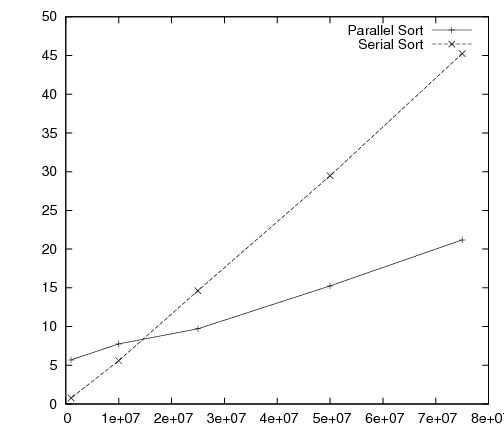
\includegraphics[width=0.6\textwidth]{img/comparison1.png}
\caption{Parallel and Serial Timing Results for Variable Array Size}
\label{chart1}
\end{figure}

\begin{figure}
\centering
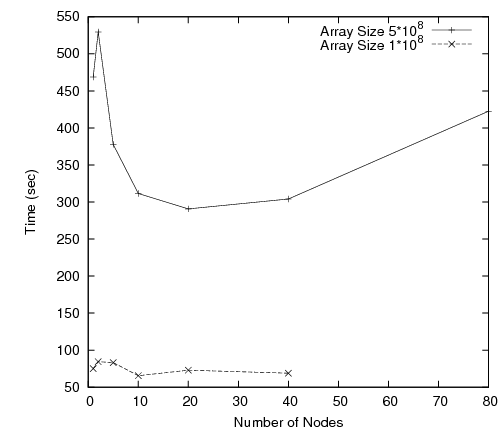
\includegraphics[width=0.6\textwidth]{img/comparison2.png}
\caption{Parallel Timing Results for Variable Node Count}
\label{chart2}
\end{figure}

Figure \ref{chart1} compares the runtime of the parallel and serial sort codes on unsorted arrays ranging from \(10^6\) to \(10^8\) elements in size. Smaller arrays sorted too quickly to be interesting and larger arrays ran into memory and message size limits. Of particular note is the fact that for problems smaller than \(10^6\) elements, the serial code is significantly faster because of the MPI startup and communications overhead. The parallel runs in Figure \ref{chart1} were run on a single quad core machine using 20 MPI nodes.

The tests in Figure \ref{chart2} were run on the cds cluster using variable numbers of nodes with both \(10^8\) data elements and \(5*10^8\) data elements. The first data point in each series, corresponding to 1 node, represents the results of the serial code. While Figure \ref{chart1} indicated that the serial code is more efficient for arrays with small numbers of data elements, Figure \ref{chart2} indicates that the serial code is also more efficient than running the parallel code on a small number of nodes. The parallel code adds extra message passing overhead which is not compensated for with enough additional processing power when only a few additional nodes are used. For both \(10^8\) data elements and \(5*10^8\) data elements, maximum efficiency of the parallel code is achieved at 10 to 20 nodes. This makes sense given that the tests were run on a 10 node cluster. Many more nodes than 10 would simply add additional communication overhead without adding additional cpu cycles.

Compared to the serial code, the parallel sort was not overwhelmingly superior. The best speedup achieved was approximately a factor of two. The parallel implementation was significantly more complicated than the serial sort (especially since the parallel sort still requires an efficient serial sort implementation). The ratio of speedup achieved to added complexity and implementation difficulty was much lower for this problem than for the n-body gravitational potential problem.


\section{Output Comparison}
\label{outputcomp}

Because this code sorts integer values, there are no floating point precision concerns like with the n-body gravitational potential problem. Thus, in every test case which I have run, the output of the parallel and serial codes have been identical.

\begin{thebibliography}{9}

\bibitem{cpl}
  Brian W. Kernighan and Dennis M. Ritchie,
  \emph{The C Programming Language},
  Prentice Hall PTR, New Jersey,
  2009.

\end{thebibliography}

\end{document}
